%
% einleitung.tex -- Beispiel-File für die Einleitung
%
% (c) 2020 Prof Dr Andreas Müller, Hochschule Rapperswil
%
% !TEX root = ../../buch.tex
% !TEX encoding = UTF-8
%
\section{Theoretische Grundlagen und Beispiele
	\label{minimalflaechen:section:Theoretische Grundlagen und Beispiele}}
\rhead{Theoretische Grundlagen und Beispiele}
Minimalflächen sind durch die Eigenschaft definiert, dass ihre mittlere Krümmung an jedem Punkt null ist.
Die mittlere Krümmung $H$ einer Fläche wird durch den Durchschnitt
%
\begin{equation}
	H=\frac{k_{1}+k_{2}}{2}
\end{equation}
%
der beiden Hauptkrümmungen $k_1$ und $k_2$ an einem Punkt berechnet.
Für Minimalflächen gilt daher
%
\begin{equation}
	k_{1}=-k_{2}.
\end{equation}

Ein weiteres charakteristisches Merkmal von Minimalflächen ist, dass sie Lösungen der Euler-Lagrange-Differentialgleichung für den Flächeninhalt darstellen.
Diese Gleichung ergibt sich aus der Bedingung, dass die erste Variation des Flächeninhalts gleich null ist.
Mathematisch wird dies durch die partielle Differentialgleichung
%
\begin{equation}
	\Delta f = 0
\end{equation}
%
ausgedrückt, wobei $\Delta$ der Laplace-Operator ist und $f$ eine Funktion, die die Fläche beschreibt.

Allerdings ist die Aussage, dass Minimalflächen die Gleichung \(\Delta f = 0\) erfüllen, nicht vollständig korrekt.
Dies gilt nur näherungsweise für Flächen, die nahezu horizontal sind.
Eine präzisere Beschreibung ergibt sich aus der nichtparametrischen Gleichung der vorgeschriebenen mittleren Krümmung.

Ist \(\mathbf{x}\) ein Graph, so schreibt er sich als

\begin{equation}
\mathbf{x}(u,v) = (u,v,\zeta(u,v))^{T}
\end{equation}
%
und die Funktion \(\zeta\) erfüllt die nichtparametrische Gleichung

\begin{equation}
(1 + \zeta_{v}^{2})\zeta_{uu} - 2\zeta_{u}\zeta_{v}\zeta_{uv} + (1 + \zeta_{u}^{2})\zeta_{vv} = H(u,v,\zeta(u,v)).
\end{equation}
%
Im Fall von Minimalflächen ist \(H = 0\) und die Gleichung wird als Minimalflächengleichung bezeichnet.
Wenn man in dieser Gleichung \(\zeta_u = \zeta_v = 0\) setzt (d.h. eine Fläche mit sehr geringer Steigung), bleibt tatsächlich nur \(\zeta_{uu} + \zeta_{vv} = \Delta \zeta\) übrig. 







\subsection{Beispiele von Minimalflächen
	\label{minimalflaechen:subsection:Beispiele von Minimalflächen}}
Es gibt viele verschiedene Arten von Minimalflächen, von denen einige besonders bekannt und gut untersucht sind.
Hier sind einige dieser Beispiele:
\begin{itemize}
	\item
	Helikoid (Wendefläche, Abbildung \ref{fig:helikoid})
	
	Diese Minimalfläche entsteht durch eine unstetige, aber isometrische Deformation des Katenoids.
	Ein Helikoid kann als eine verallgemeinerte Spirale betrachtet werden.
	Die Gleichung, die ein Helikoid beschreibt, ist $z=\theta$, wobei $\theta$ der Winkel in Zylinderkoordinaten ist.
	%
	Das Helikoid ist wie eine Wendeltreppe, welche sich in einer endlosen Spirale nach oben und unten wendet.
	%
\begin{figure}
	\centering
	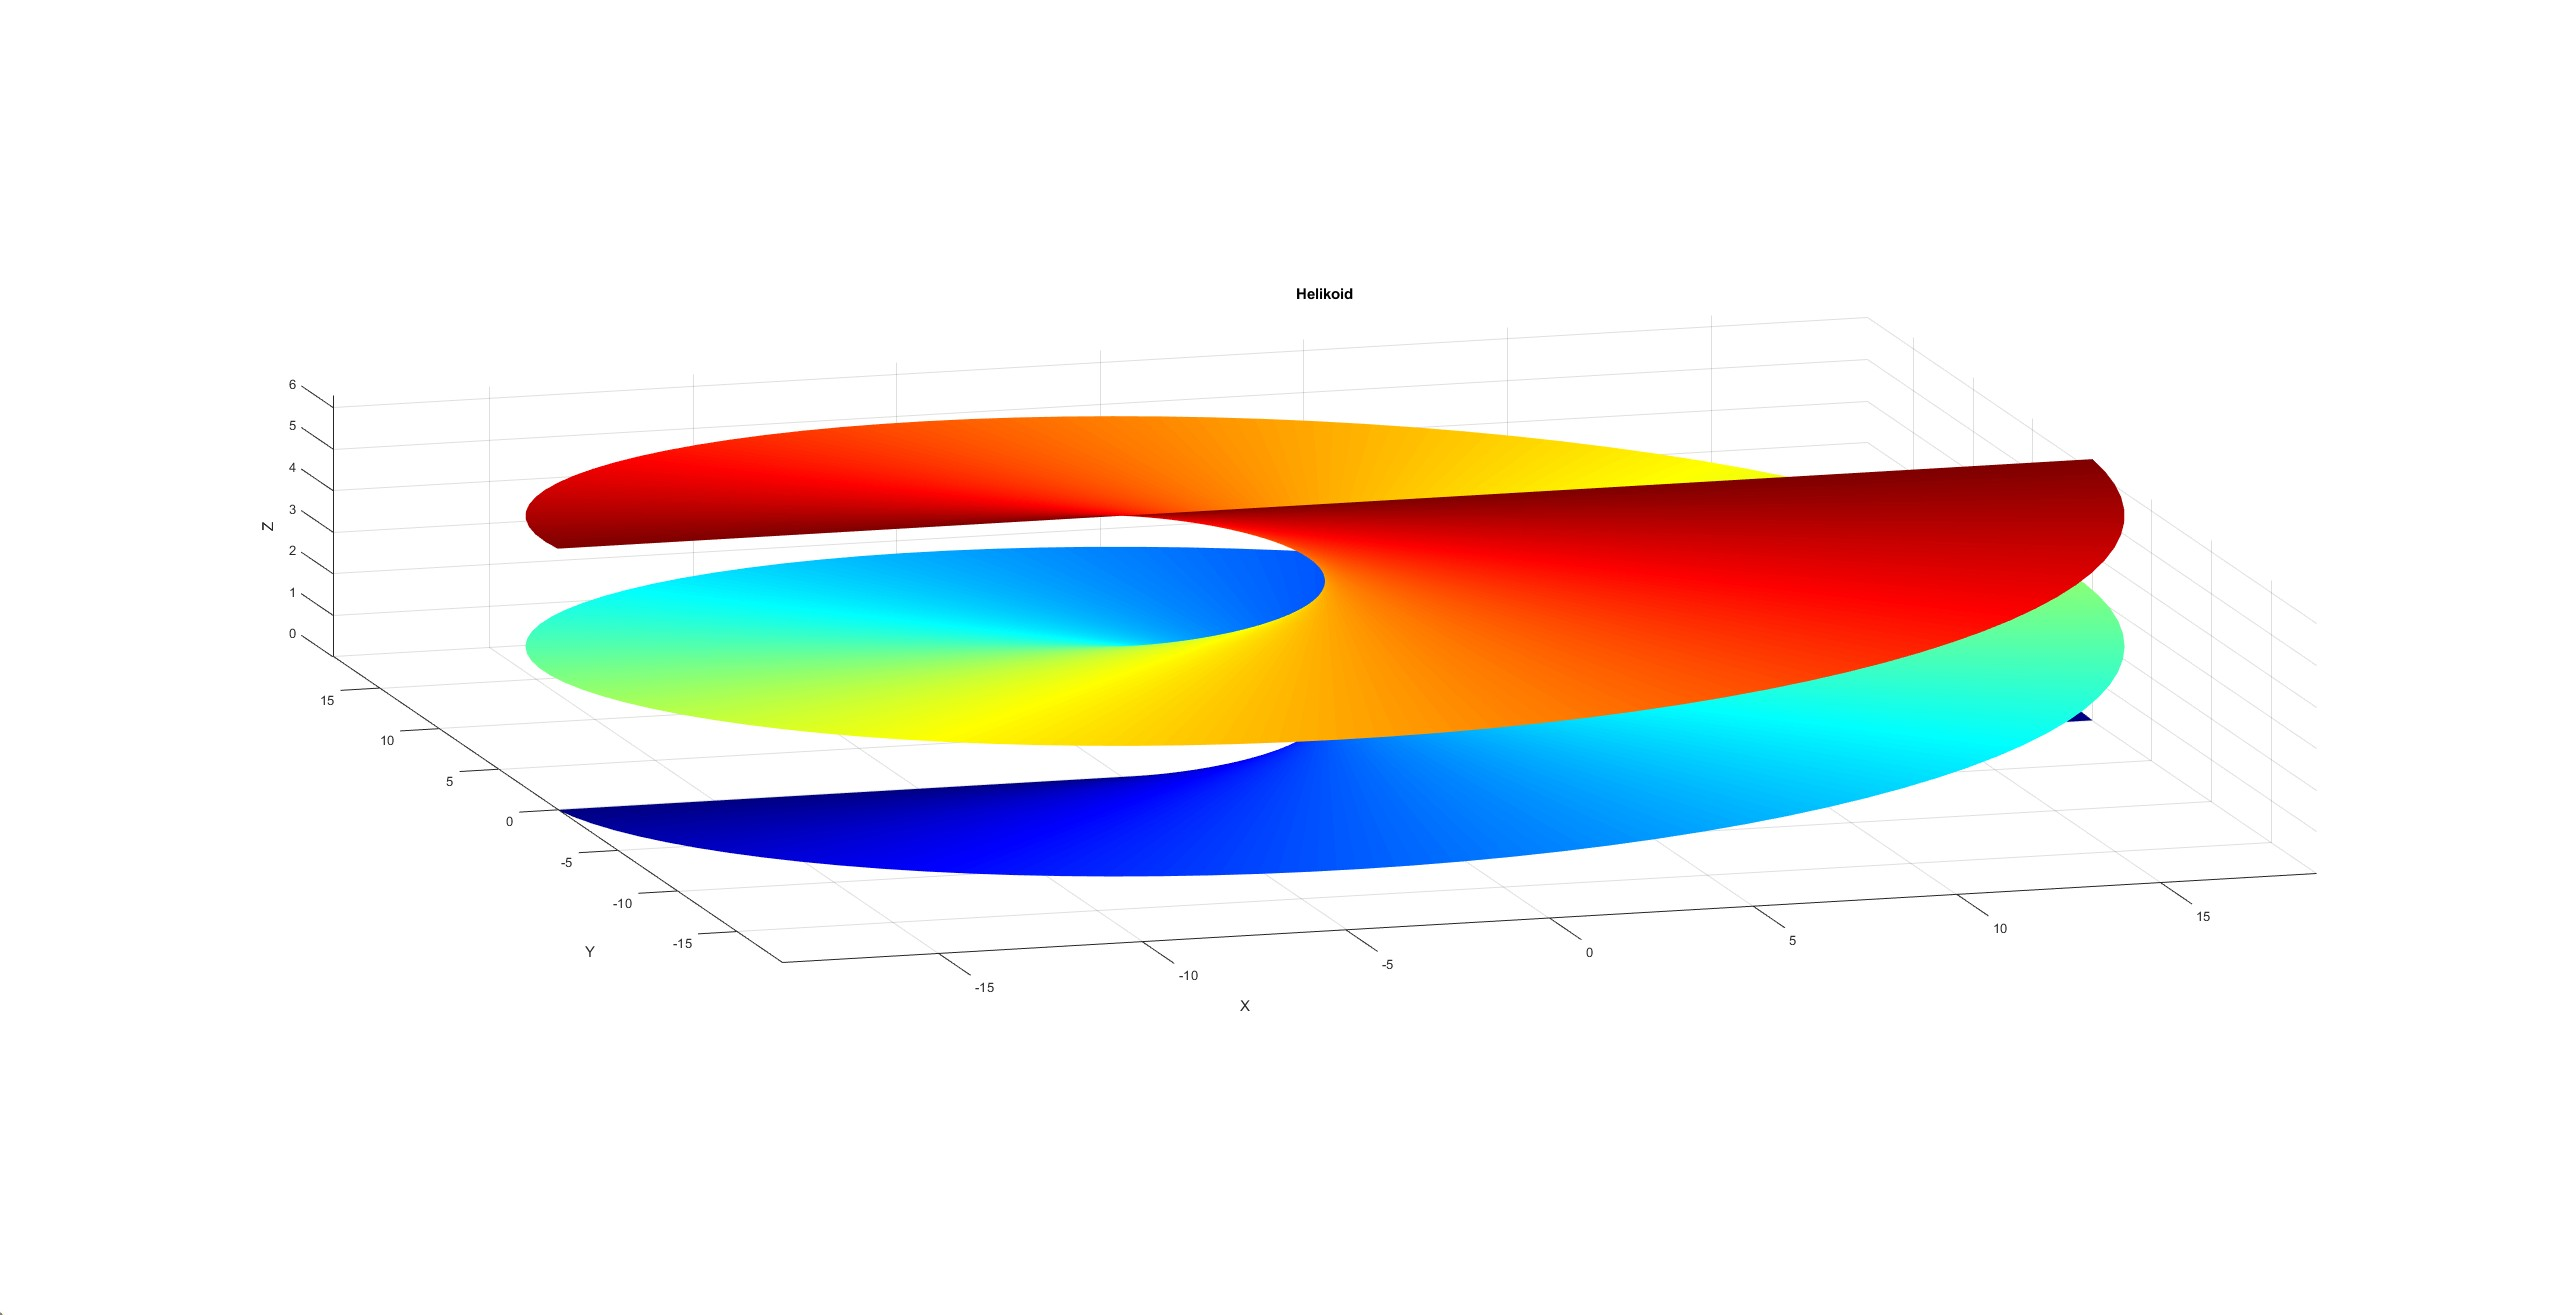
\includegraphics[width=\textwidth]{papers/minimalflaechen/Helikoid}
	\caption{Helikoid}
	\label{fig:helikoid}
\end{figure}

	\item
	Katenoid
	
	Das Katenoid ist eine Rotationsfläche, welche durch die Drehung einer Kettenlinie um die $x$-Achse entsteht.
	Sie ist die einzige Minimalfläche, die auch eine Rotationsfläche ist.
	Eine Kettenlinie ist die Kurve, die durch eine ideale flexible Kette oder ein Seil gebildet wird, welche unter dem Einfluss der Schwerkraft hängt.
	Das Katenoid ist eine der einfachsten und bekanntesten Minimalflächen.
	
	Unter diesem Link \url{https://www.geogebra.org/m/BtAdpcYM} kann man sehen, wie durch die Rotation einer Kettenlinie ein Katenoid entsteht.
	\item
	Scherk'sche Minimalfläche (Abbildung \ref{fig:schreksche-minimalflache})
	
	Diese Minimalfläche wurde von Heinrich Ferdinand Scherk im Jahr 1834 entdeckt.
	Sie hat eine schachbrettartige Struktur und wird durch die Gleichung 
	\begin{equation}
		z=\ln(\frac{\cos(y)}{\cos(x)}) 
	\end{equation}
	beschrieben.
%
\begin{figure}
	\centering
	\includegraphics[width=0.7\linewidth]{"papers/minimalflaechen/doublyscherkshear"}
	\caption{Scherk'sche Minimalfläche \cite{minimalflaechen:doublyscherkshear}}
	\label{fig:schreksche-minimalflache}
\end{figure}
	\item
	Henneberg-Fläche (Abbildung \ref{fig:henneberg-flache})
	
	Diese nicht orientierbare Minimalfläche wurde von Ernst Lebrecht Henneberg entdeckt.
\begin{figure}
	\centering
	\includegraphics[width=0.7\linewidth]{"papers/minimalflaechen/Henneberg Fläche"}
	\caption{Henneberg Fläche \cite{minimalflaechen:henneberg}}
	\label{fig:henneberg-flache}
\end{figure}

Man stelle sich eine Ameisenkolonie vor, die auf dieser Fläche herumkrabbelt.
Da diese Fläche keine eindeutige Normalenrichtung hat, könnten die Ameisen, ohne es zu bemerken, auf der anderen Seite der Fläche wieder auftauchen, nachdem sie eine Schleife gelaufen sind.
Es ist, als ob sie in einer vierdimensionalen Welt unterwegs wären, in der Oben und Unten, Innen und Aussen keine festen Begriffe mehr sind.


\end{itemize}

\subsection{Anwendungen von Minimalflächen
	\label{minimalflaechen:subsection:Anwendungen von Minimalflächen}}
Minimalflächen haben zahlreiche Anwendungen in der realen Welt.
In der Architektur und im Bauwesen werden sie genutzt, um stabile und ästhetisch ansprechende Strukturen zu entwerfen.
Ihre Eigenschaft, die Fläche zu minimieren, macht sie ideal für Konstruktionen, die leicht werden müssen und damit weniger Material brauchen.

Ein bekanntes Beispiel für die Anwendung von Minimalflächen in der Architektur ist das Münchner Olympiastadion (Abbildung \ref{fig:stadion-1}).
Das Dach dieses Stadions basiert auf Prinzipien von Minimalflächen und zeigt, wie solche Flächen genutzt werden können, um beeindruckende und funktionale Bauwerke zu schaffen.
Durch die Minimierung der Fläche wird nicht nur Material gespart, sondern auch eine elegante und leichte Struktur geschaffen, die dennoch stabil und langlebig ist.
\begin{figure}
	\centering
	\includegraphics[width=\textwidth]{"papers/minimalflaechen/Stadion 1"}
	\caption{Olympiastadion München \cite{minimalflaechen:Olympiastadion}}
	\label{fig:stadion-1}
\end{figure}


Ein alltägliches Beispiel für eine Minimalfläche ist eine Seifenblase.
Wenn man einen Draht in eine Seifenlösung taucht und dann herauszieht, bildet sich zwischen den Drähten eine dünne Seifenhaut, die eine Minimalfläche darstellt.
Diese Seifenhaut strebt danach, ihre Oberfläche zu minimieren und so die Fläche zwischen den Drähten so klein wie möglich zu halten.
Die Kräfte, die auf die Seifenhaut wirken, sorgen dafür, dass sie diese minimale Fläche einnimmt.

